\documentclass[12pt]{article}
\usepackage[utf8]{inputenc}
\usepackage{graphicx} % Allows you to insert figures
\usepackage{amsmath} % Allows you to do equations
\usepackage{fancyhdr} % Formats the header
\usepackage{geometry} % Formats the paper size, orientation, and margins
\linespread{1.25} % about 1.5 spacing in Word
\setlength{\parindent}{0pt} % no paragraph indents
\setlength{\parskip}{1em} % paragraphs separated by one line
\usepackage[format=plain,
            font=it]{caption} % Italicizes figure captions
\usepackage[english]{babel}
\usepackage{csquotes}
\renewcommand{\headrulewidth}{0pt}
\geometry{letterpaper, portrait, margin=1in}
\setlength{\headheight}{14.49998pt}
\geometry{a4paper, left=20mm, right=20mm, top=35mm, bottom=20mm}

\newcommand\titleofdoc{\LARGE{\textbf{Assignment-8: Digital Fourier Transform}}}
\newcommand\GroupName{EE20B136}

\begin{document}
\begin{titlepage}
   \begin{center}
        \vspace*{4cm} % Adjust spacings to ensure the title page is generally filled with text

        \Huge{\titleofdoc} 

        \vspace{3 cm}
        \Large{Syam SriBalaji T}
       
        \vspace{0.25cm}
        \large{EE20B136}
       
        \vspace{3 cm}
        \Large{April 17, 2022}
        
        \vspace{0.25 cm}
        \Large{EE2703 :Jan-May 2022}
       

       \vfill
    \end{center}
\end{titlepage}

\setcounter{page}{2}
\pagestyle{fancy}
\fancyhf{}
\rhead{\thepage}

\section*{Spectrum of $sin^3(t)$:}

Firstly, let us expand $sin^3(t)$, we get
\begin{equation*}
sin^3(t)=\frac{3sin(t)-sin(3t)}{4}
\end{equation*}
\\
So, for $sin^3(t)$ we should expect 4 impulses in DFT magnitude plot, while 2 impulses(with same amplitude) being thrice the amplitude of other 2 impulses(with same amplitude). And also the 2 impulses(with same amplitude) will have phases with opposite sign but same magnitude, in both case.

So, same as our anticipation, here is the DFT Amplitude and Phase plot of $sin^3(t)$, 
\begin{figure}[h!]
\centering
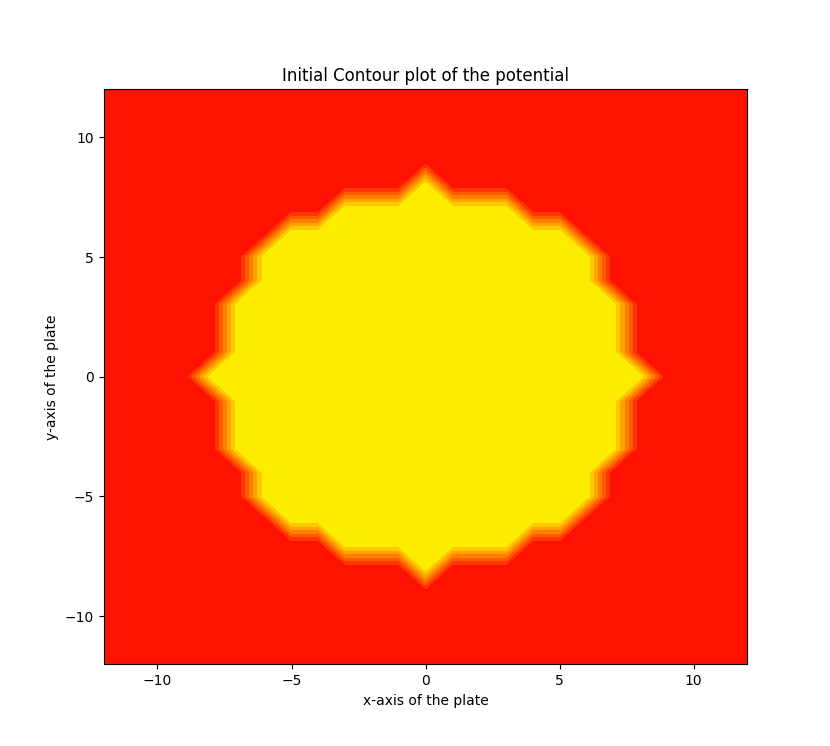
\includegraphics[height=12cm]{Figure_1.png}
\end{figure}

\newpage
\section*{Spectrum of $cos^3(t)$:}

Firstly, let us expand $cos^3(t)$, we get

\begin{equation*}
cos^3(t) = \frac{cos(3t)+3cos(t)}{4}
\end{equation*}
\\
So, for $cos^3(t)$ also, we should expect 4 impulses in DFT magnitude plot, where 2 impulses(with same amplitude) being thrice the amplitude of other 2 impulses(with same amplitude). And notably all the 4 impulses will have same zero phase magnitude.

So, same as our anticipation, here is the DFT Amplitude and Phase plot of $cos^3(t)$, 
\begin{figure}[h!]
\centering
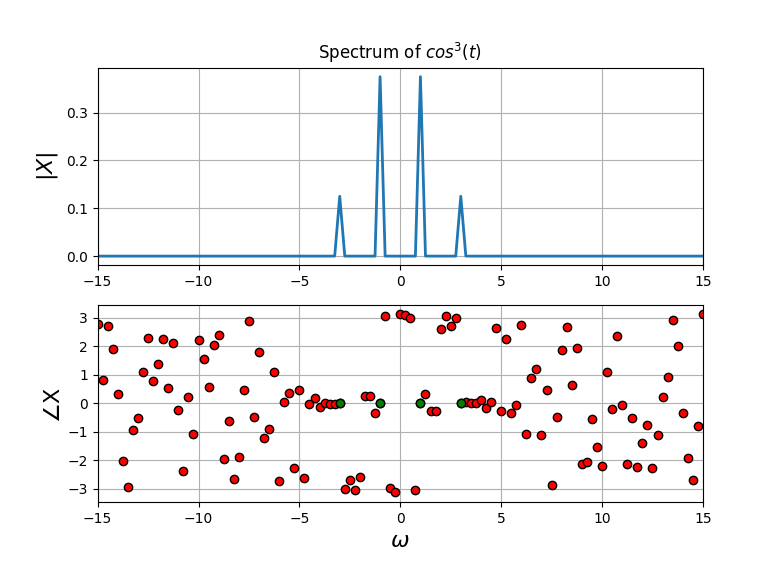
\includegraphics[height=12cm]{Figure_2.png}
\end{figure}

\newpage
\section*{Spectrum of $cos(20t +5.cos(t))$:}

The Equation is $cos(20t +5.cos(t))$, in which cosine itself consists of cosine, so it is a Frequency Modulation function. We can expect large number of impulse, thus we need large number of points(i.e. 512) in between them to get the accurate graph.\\\\

If the same equation is expressed in Bessel function, we will get frequency spectrum with impulses at carrier frequency(i.e. $\omega_{c}=|20|$) and several other impulses with multiple side band frequencies on either sides, which is close to carrier frequency.\\\\

 As our expectation, here is the DFT Amplitude and Phase plot of $cos(20t +5.cos(t))$:

\begin{figure}[h!]
\centering
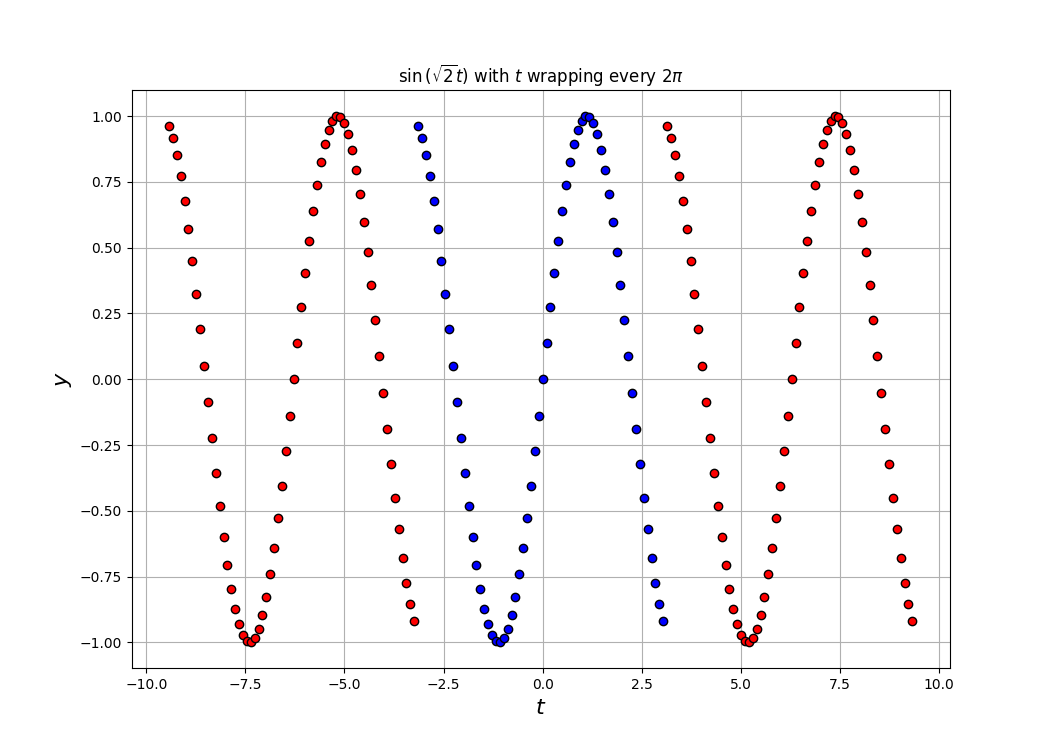
\includegraphics[height=12cm]{Figure_3.png}
\label{fig:exemplo}
\end{figure}

Here we can also notice that the magnitude of phase at carrier frequency on each side of the phase plot(+ve and -ve frequency side) are in opposite sign. Likewise for every other impulses. 

\newpage
\section*{Gaussian Exponential Function   $e^{(-t^2/2)}$:}

The function 
\begin{equation*}
f(x)=e^{(-t^2/2)}
\end{equation*}
is not frequency Band-limited(the frequency spectrum will have non-zero values for even beyond cut-off frequencies). And we calculate DFT of this equation, we get
\begin{equation*}
F(\omega)=\frac{1}{\sqrt{2\pi}}\times e^{(-\omega^2/2)}
\end{equation*}
\\And we will estimate the error by finding difference between both. To find the best estimated graph, we need to find the graph with least error. So we should plot for different range $(-r\pi,r\pi)$ and different Number of points in between them(N).\\\\
Here we have variety of plots and let's search for plot with minimum error.

\begin{figure}[h!]
\centering
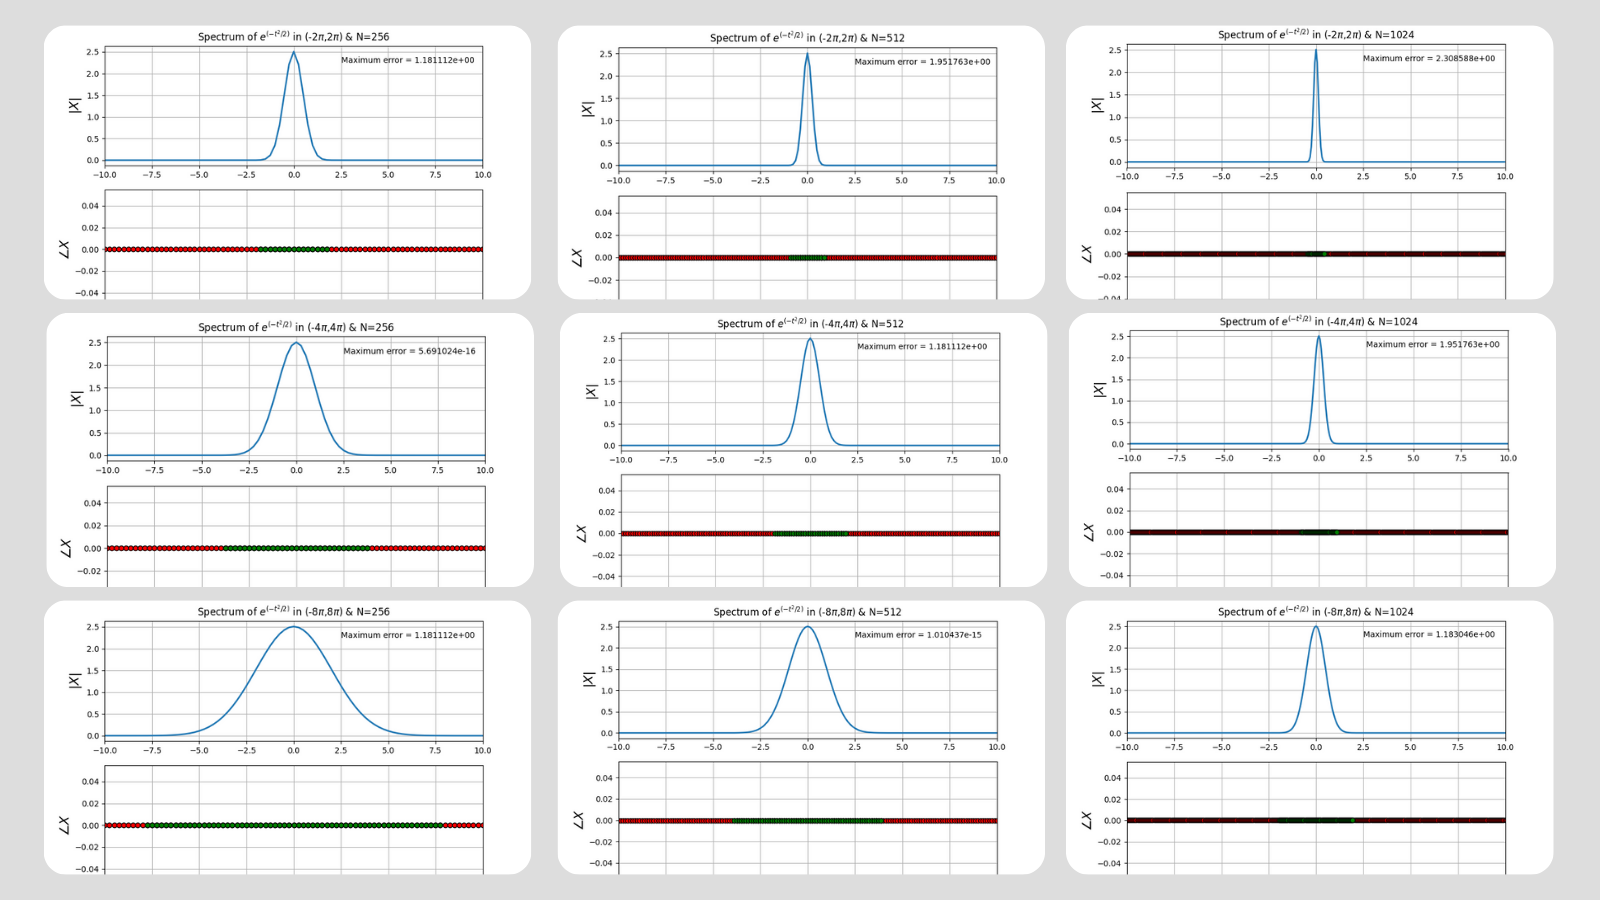
\includegraphics[height=10cm]{grid.png}
\label{fig:exemplo}
\end{figure}

\newpage
\section*{Spectrum of $e^{(-t^2/2)}$ with Maximum accuracy:}

So, from the above set plots, we notice that the Spectrum of $e^{(-t^2/2)}$ is having Maximum accuracy for range (-4$\pi$,4$\pi$) and N=256, with $error= 5.691024\times 10^{-16}$.
\begin{figure}[h!]
\centering
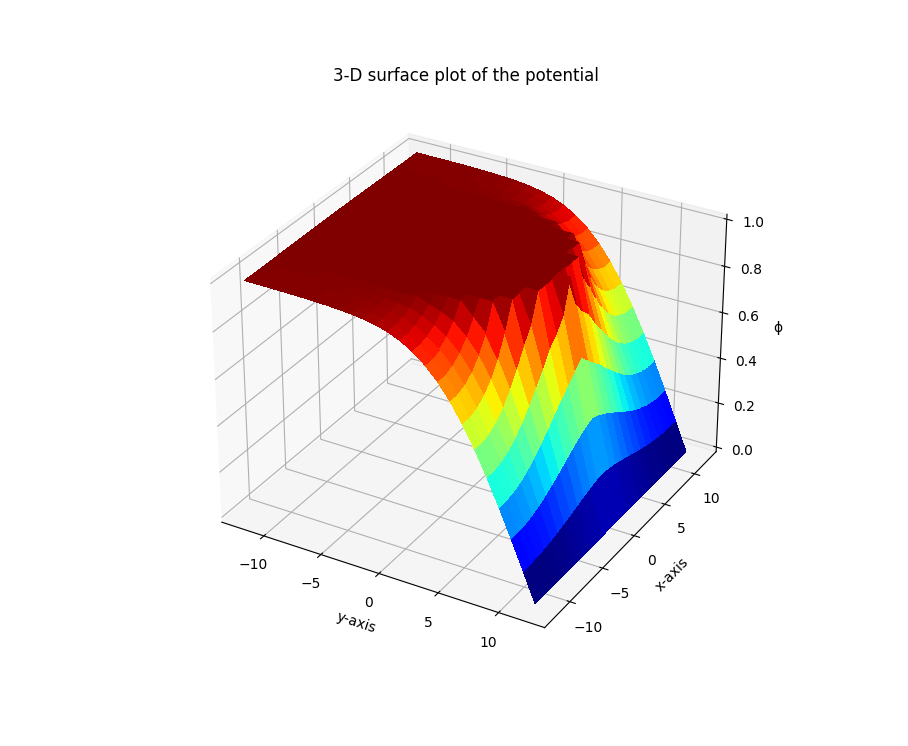
\includegraphics[height=12cm]{Figure_7.png}
\label{fig:exemplo}
\end{figure}

\section*{\textbf{Conclusion:}}
The functions like $'fft'$ , $'fftshift'$ from numpy library eases the job of creating DFT of functions. Almost making us possible to create DFT's for any desired function in python with more accuracy. Thus, makes python more powerful.

\begin{center} 
\textbf{Thank you!}
\end{center} 
\end{document}
